
\section{proteins.xml, rnas.xml and dna.xml}

All these files are base on the same class \rbamacromolecules.

\subsection{Rationale}

In RBA, basic molecules are seen either as metabolites or macromolecules.
In the current version, macromolecules encompass the polymer molecules
proteins, RNAs and DNA.
In future versions, we would like to extend the definition to other molecules
that have polymer-like properties in their assembly process (e.g. lipids).

The formal distinction between macromolecules and other molecules is that
macromolecules can be defined as an ensemble of other, simpler
molecules or molecule residues.
Elements of a macromolecule family (proteins, RNAs, DNA) are based on the same subset of
component molecules (amino acid residues, vitamins, ions for proteins),
share common assembly processes,
but differ in the stoichiometry of components they are built of.

For example, a protein is often described as a sequence of letters, say
"MAGLKYAAALK",
where every letter implicitly represents a component (an amino acid residue).
It may also contain post-translational modifications,
such as a phosphorylation on the tyrosine Y.
The RBA format starts by listing the components that are common to all proteins:
all amino acid residues (A, C, .., Y), vitamins, ions and other cofactors.
The second part of the RBA format lists all proteins broken down as an ensemble
of components.
For example, the protein above would be described as
\{(A:4), (G:1), (K:2), (L:2), (M:1), (Y:1), (Phospho:1)\},
where Phospho represents the tyrosine phosphorylation
(in this example, we pooled all possible phosphorylations into a single component).

Note that macromolecule components are \emph{not} metabolites.
How they are built from metabolites is part of the assembly process defined in
processes.xml.
They may share identical identifiers as metabolites, but we advise using different
identifiers for clarity.
For example, an amino acid residue is \emph{not} an amino acid:
it is obtained by loading a charged tRNA onto a nascent protein with the appropriate
energetic molecules, while releasing several byproducts, including an uncharged tRNA.
In a sense, a component can be seen as an \emph{atomic assembly action},
rather than a submolecule.

The macromolecule files contain static descriptions of the macromolecules.
How they are assembled from metabolites and the machines needed to assemble
them are defined in processes.xml.

\subsection{RBAMacromolecules}
\label{sec:rba_macromolecules}

The outermost part of the protein, RNA and DNA files is an instance of class
\rbamacromolecules, shown in Figure~\ref{fig:macromolecules}.

\begin{figure}
  \centering
  \includegraphics[scale=0.8]{figures/macromolecules}
  \caption{XML structure of macromolecule document.}
\label{fig:macromolecules}
\end{figure}

\rbamacromolecules{} has no simple attributes.
It contains exactly one instance of \textbf{ListOfComponents}
and \textbf{ListOfMacromolecules}.


\subsection{Component}
\label{sec:component}

The \component{} class is used to define the components of a \macromolecule{}
(Fig.~\ref{fig:macromolecules}).
For example, these are expected to be amino acids, vitamins and ions for
proteins.
Even if there is a strong connection between metabolic \species{} and \component{}s,
they are seen as independent entities with separate identifiers.
The connection between \species{} and \component{}s is established in the process file,
where \processingmap{}s define how components are assembled from metabolites.


\paragraph{The \textit{id} attribute}
The \textbf{id} attribute is a string defining the identifier of a component.

\paragraph{The \textit{weight} attribute}
The \textbf{weight} attribute is a real number defining the weight of a
component.
This information is essential for the density constraints.
The weight of a macromolecule is defined as the sum of the weight of its
components.
The weight unit is unspecified, however it should be consistent with the parameters
used in the density constraints.

\paragraph{The \textit{name} and \textit{type} attributes}
The \textbf{name} and \textbf{type} attributes are strings that provide
additional information about the component.
The name is a standard name of the component
(\textit{e.g.} full amino acid name).
The type can be used to distinguish components if necessary
(\textit{e.g.} in amino acids, vitamins, ions).


\subsection{Macromolecule}
\label{sec:macromolecule}

The \macromolecule{} class is used to define macromolecular species
(Fig.~\ref{fig:macromolecules}).
Its composition is given by a \textbf{ListOfComponentReferences}.

\paragraph{The \textit{id} attribute}
The \textbf{id} attribute is a string defining the identifier of
the macromolecule.

\paragraph{The \textit{compartment} attribute}
The \textbf{compartment} attribute must match the identifier of a \compartment.
It represents the compartment where the molecule is thought to be active.


\subsection{ComponentReference}
\label{sec:component_reference}

The \componentreference{} class is used to refer to a \component{}
and associate with it a stoichiometry (Fig.~\ref{fig:macromolecules}).

\paragraph{The \textit{component} attribute}
The \textbf{component} attribute must match the identifier of a \component{}
defined in the same \rbamacromolecules{} instance.

\paragraph{The \textit{stoichiometry} attribute}
The \textbf{stoichiometry} is a positive real number.
It represents the stoichiometry of a \component{}
(typically how often it appears in a \macromolecule,
e.g.\ the number of alanine residues in a protein).

\subsection{Examples}

The list of components and complexity of macromolecule definitions depends on
the desired level of detail.
In real models, we include a large list of possible components including all
amino acid residues and cofactors for proteins (Fig.~\ref{fig:proteins_ex_1}).
In processes.xml, we will define how each component is built from metabolites.
In particular, a protein can only be built if all components can be assembled,
including cofactors.
For example, BSU29470 cannot be produced in the absence of magnesium.
Note that in this model, we consider that all amino acid residues have a weight
of 1, while cofactors have a weight of 0.
This is a simplifying assumption that enables us to estimate the overall weight
of proteins in the model.
We consider that this level of granularity is sufficient to define density
constraints at a satisfactory resolution.

In our minimal model (Fig.~\ref{fig:proteins_ex_2}),
we consider that all proteins are made of a single component that more or less
represents all amino acid residues, there is no cofactor.
We only define two proteins with different lengths for illustration purposes.
In comparison, the real model contains several thousands of proteins.

\begin{figure}
  \centering
  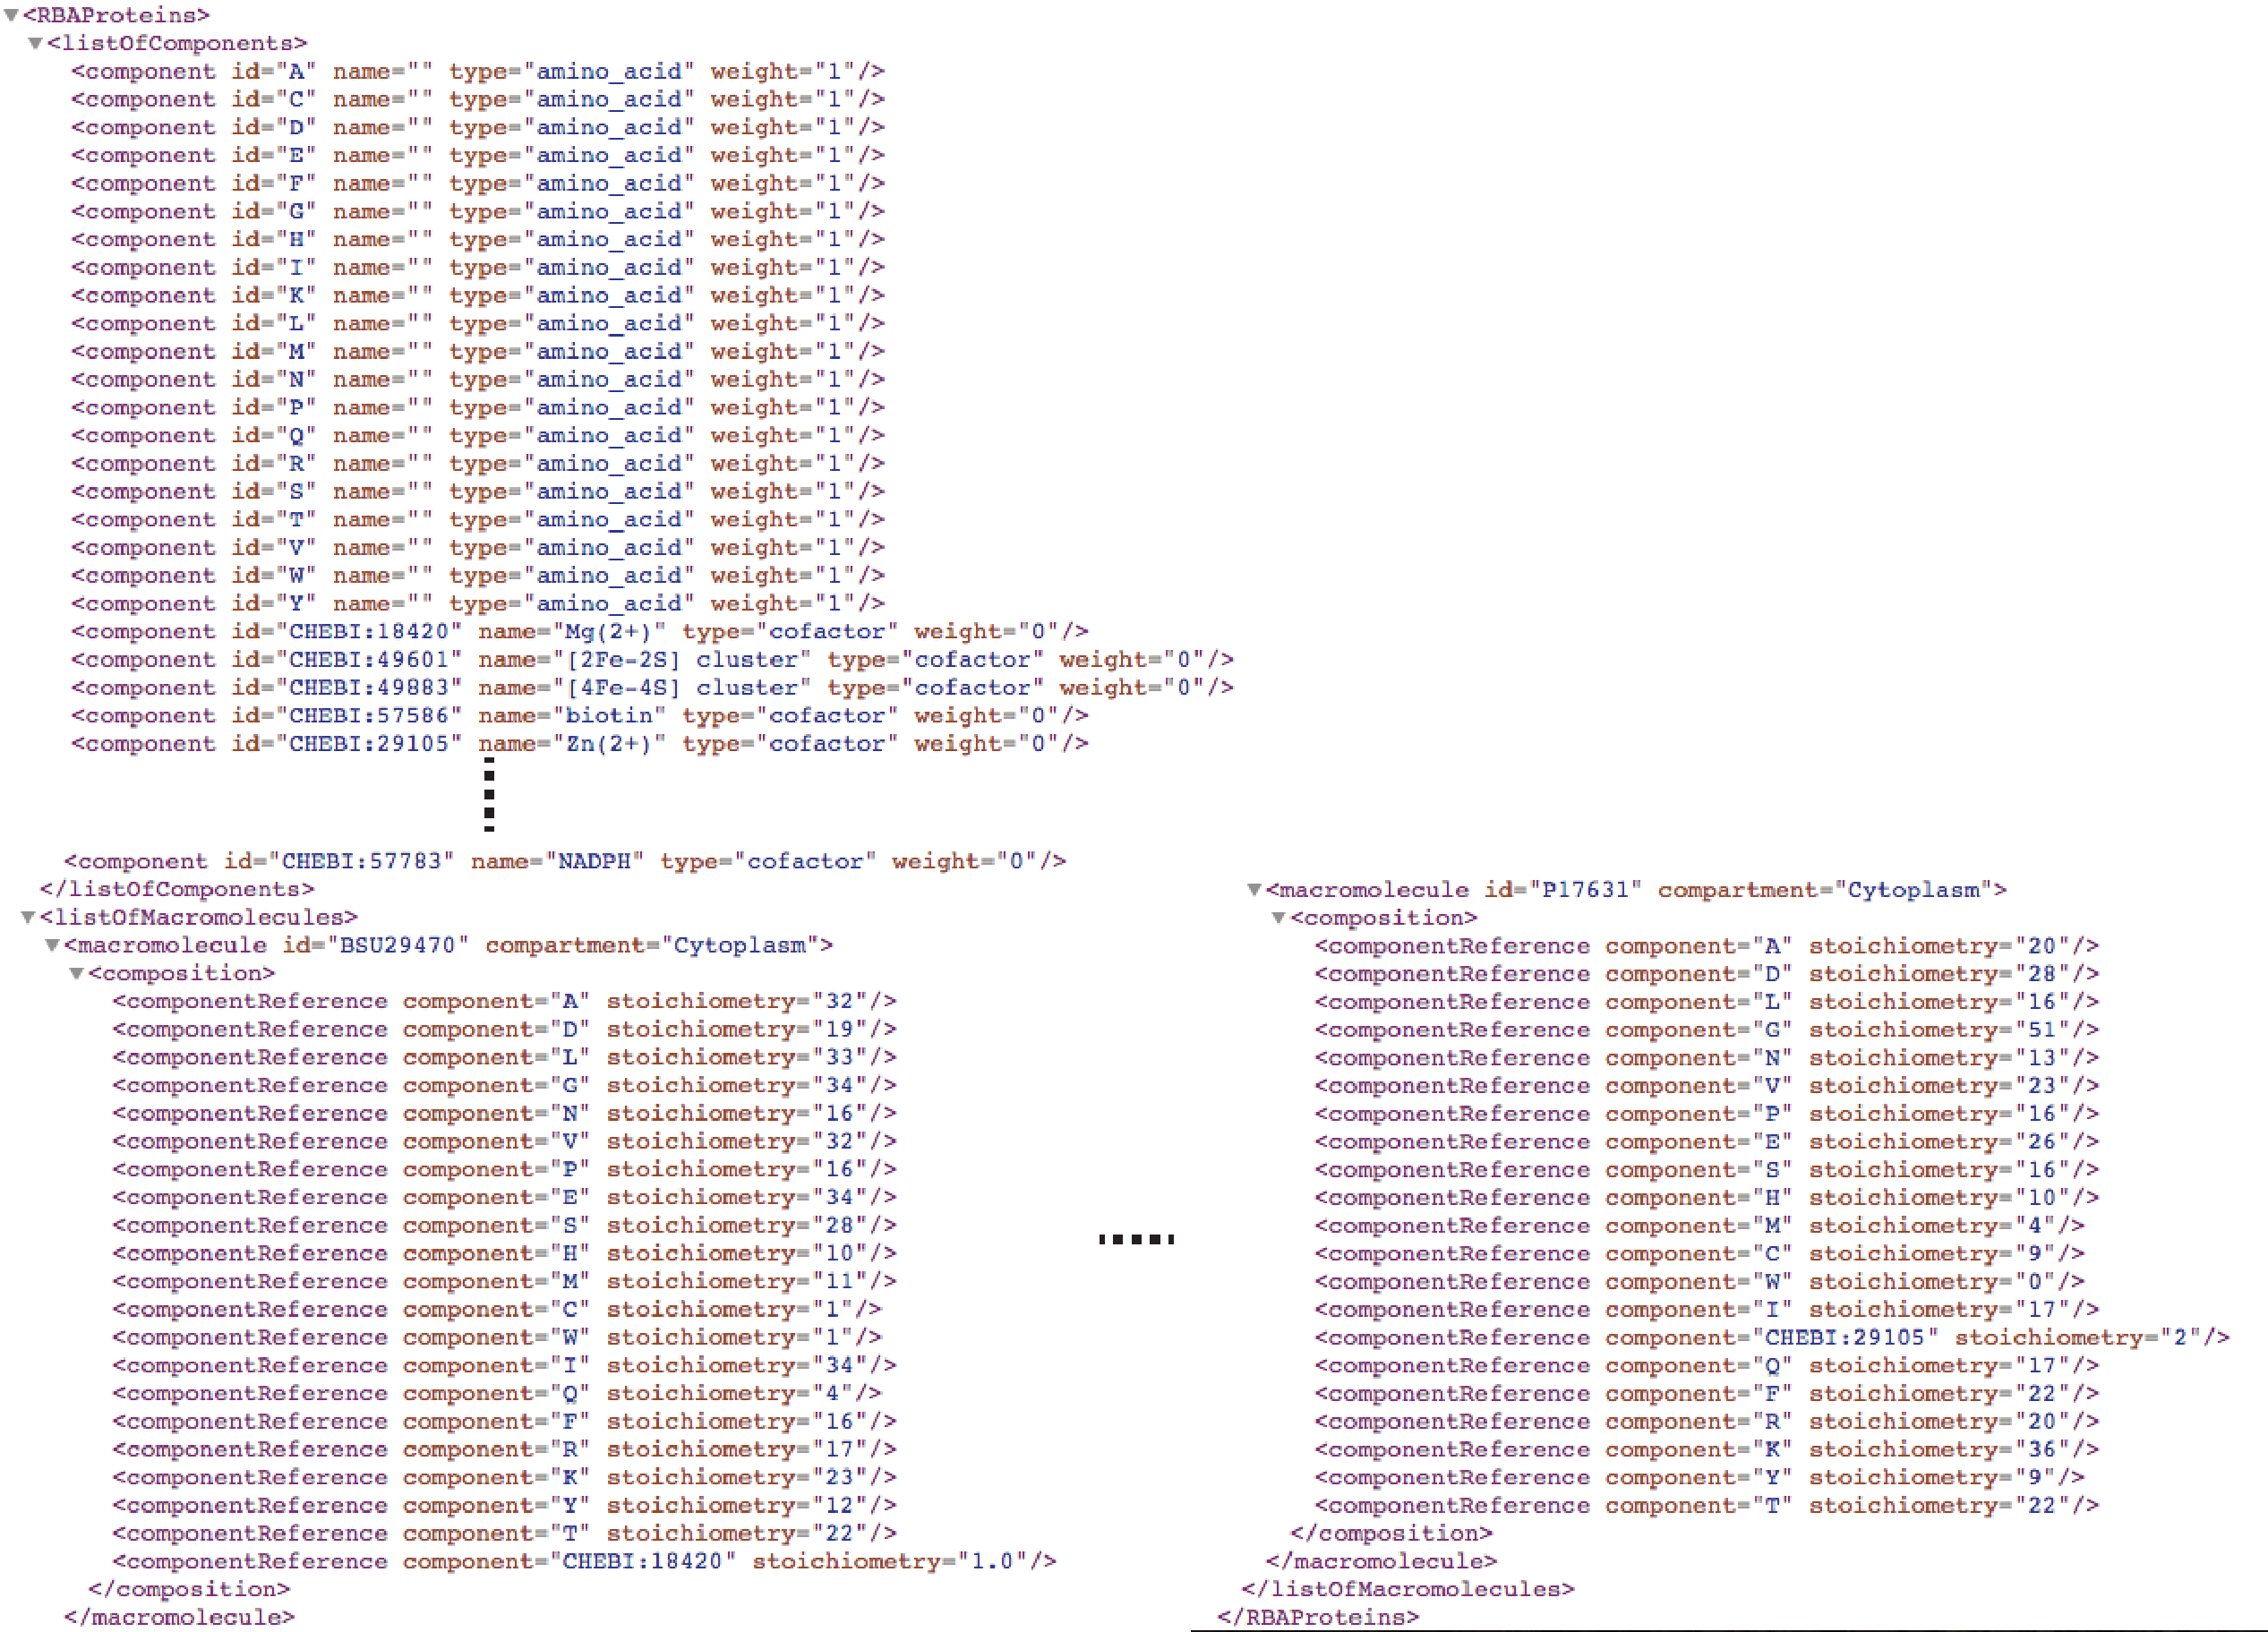
\includegraphics[scale=0.4]{figures/proteins_ex_1}
  \caption{proteins.xml from the model automatically generated by RBApy for the
  model bacteria \textit{B. subtilis}. Large chunks of the files were removed
  for brevity. The file contains two lists.
  The component list contains construction blocks for proteins: amino acid
  residues and cofactors such as ions and vitamins.
  The macromolecule list defines all the proteins in the system.
  Here we show two examples of cytosolic proteins, defined as an ensemble of
  amino acid residues and cofactors.}
  \label{fig:proteins_ex_1}
\end{figure}

\begin{figure}
  \centering
  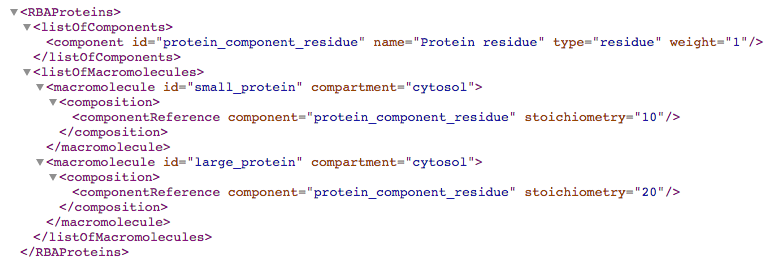
\includegraphics[scale=0.6]{figures/proteins_ex_2}
  \caption{proteins.xml from the minimal model.
  In the minimal model, we do not detail every amino acid residue, we just
  consider that proteins contain different amounts of a
  "protein\_component\_residue".}
  \label{fig:proteins_ex_2}
\end{figure}
